\section{Discussion: example cases}

\label{sec_lptdiscussion}

Finally, we can perform numerical simulation for multiphase flows, including:

\begin{itemize}
  \item {continuous phase (liquid/gas, etc)}, 
  \item {discrete phase (particle/droplet, etc)}.
\end{itemize}

Various multiphase examples were simulated with {\psiboil}.
In this section, four cases are discussed, including:

\begin{itemize}
  \item {T-Junction particle deposition rate}, 
  \item {One-dimensional particle deposition on dispersed surface},
  \item {Terminal velocity verification},
  \item {Particle deposition of multiphase flow}.
\end{itemize}

\subsection{T-Junction particle deposition rate}

%------------------%
%                  %
%  model and mesh  %
%                  %
%------------------%
\begin{figure}[ht]
  \centering
  \setlength{\unitlength}{ 1mm}
  \begin{picture}( 70, 50)( 0, 0)
    \thickbox{ 70}{ 50}
    %\put( 0, 0){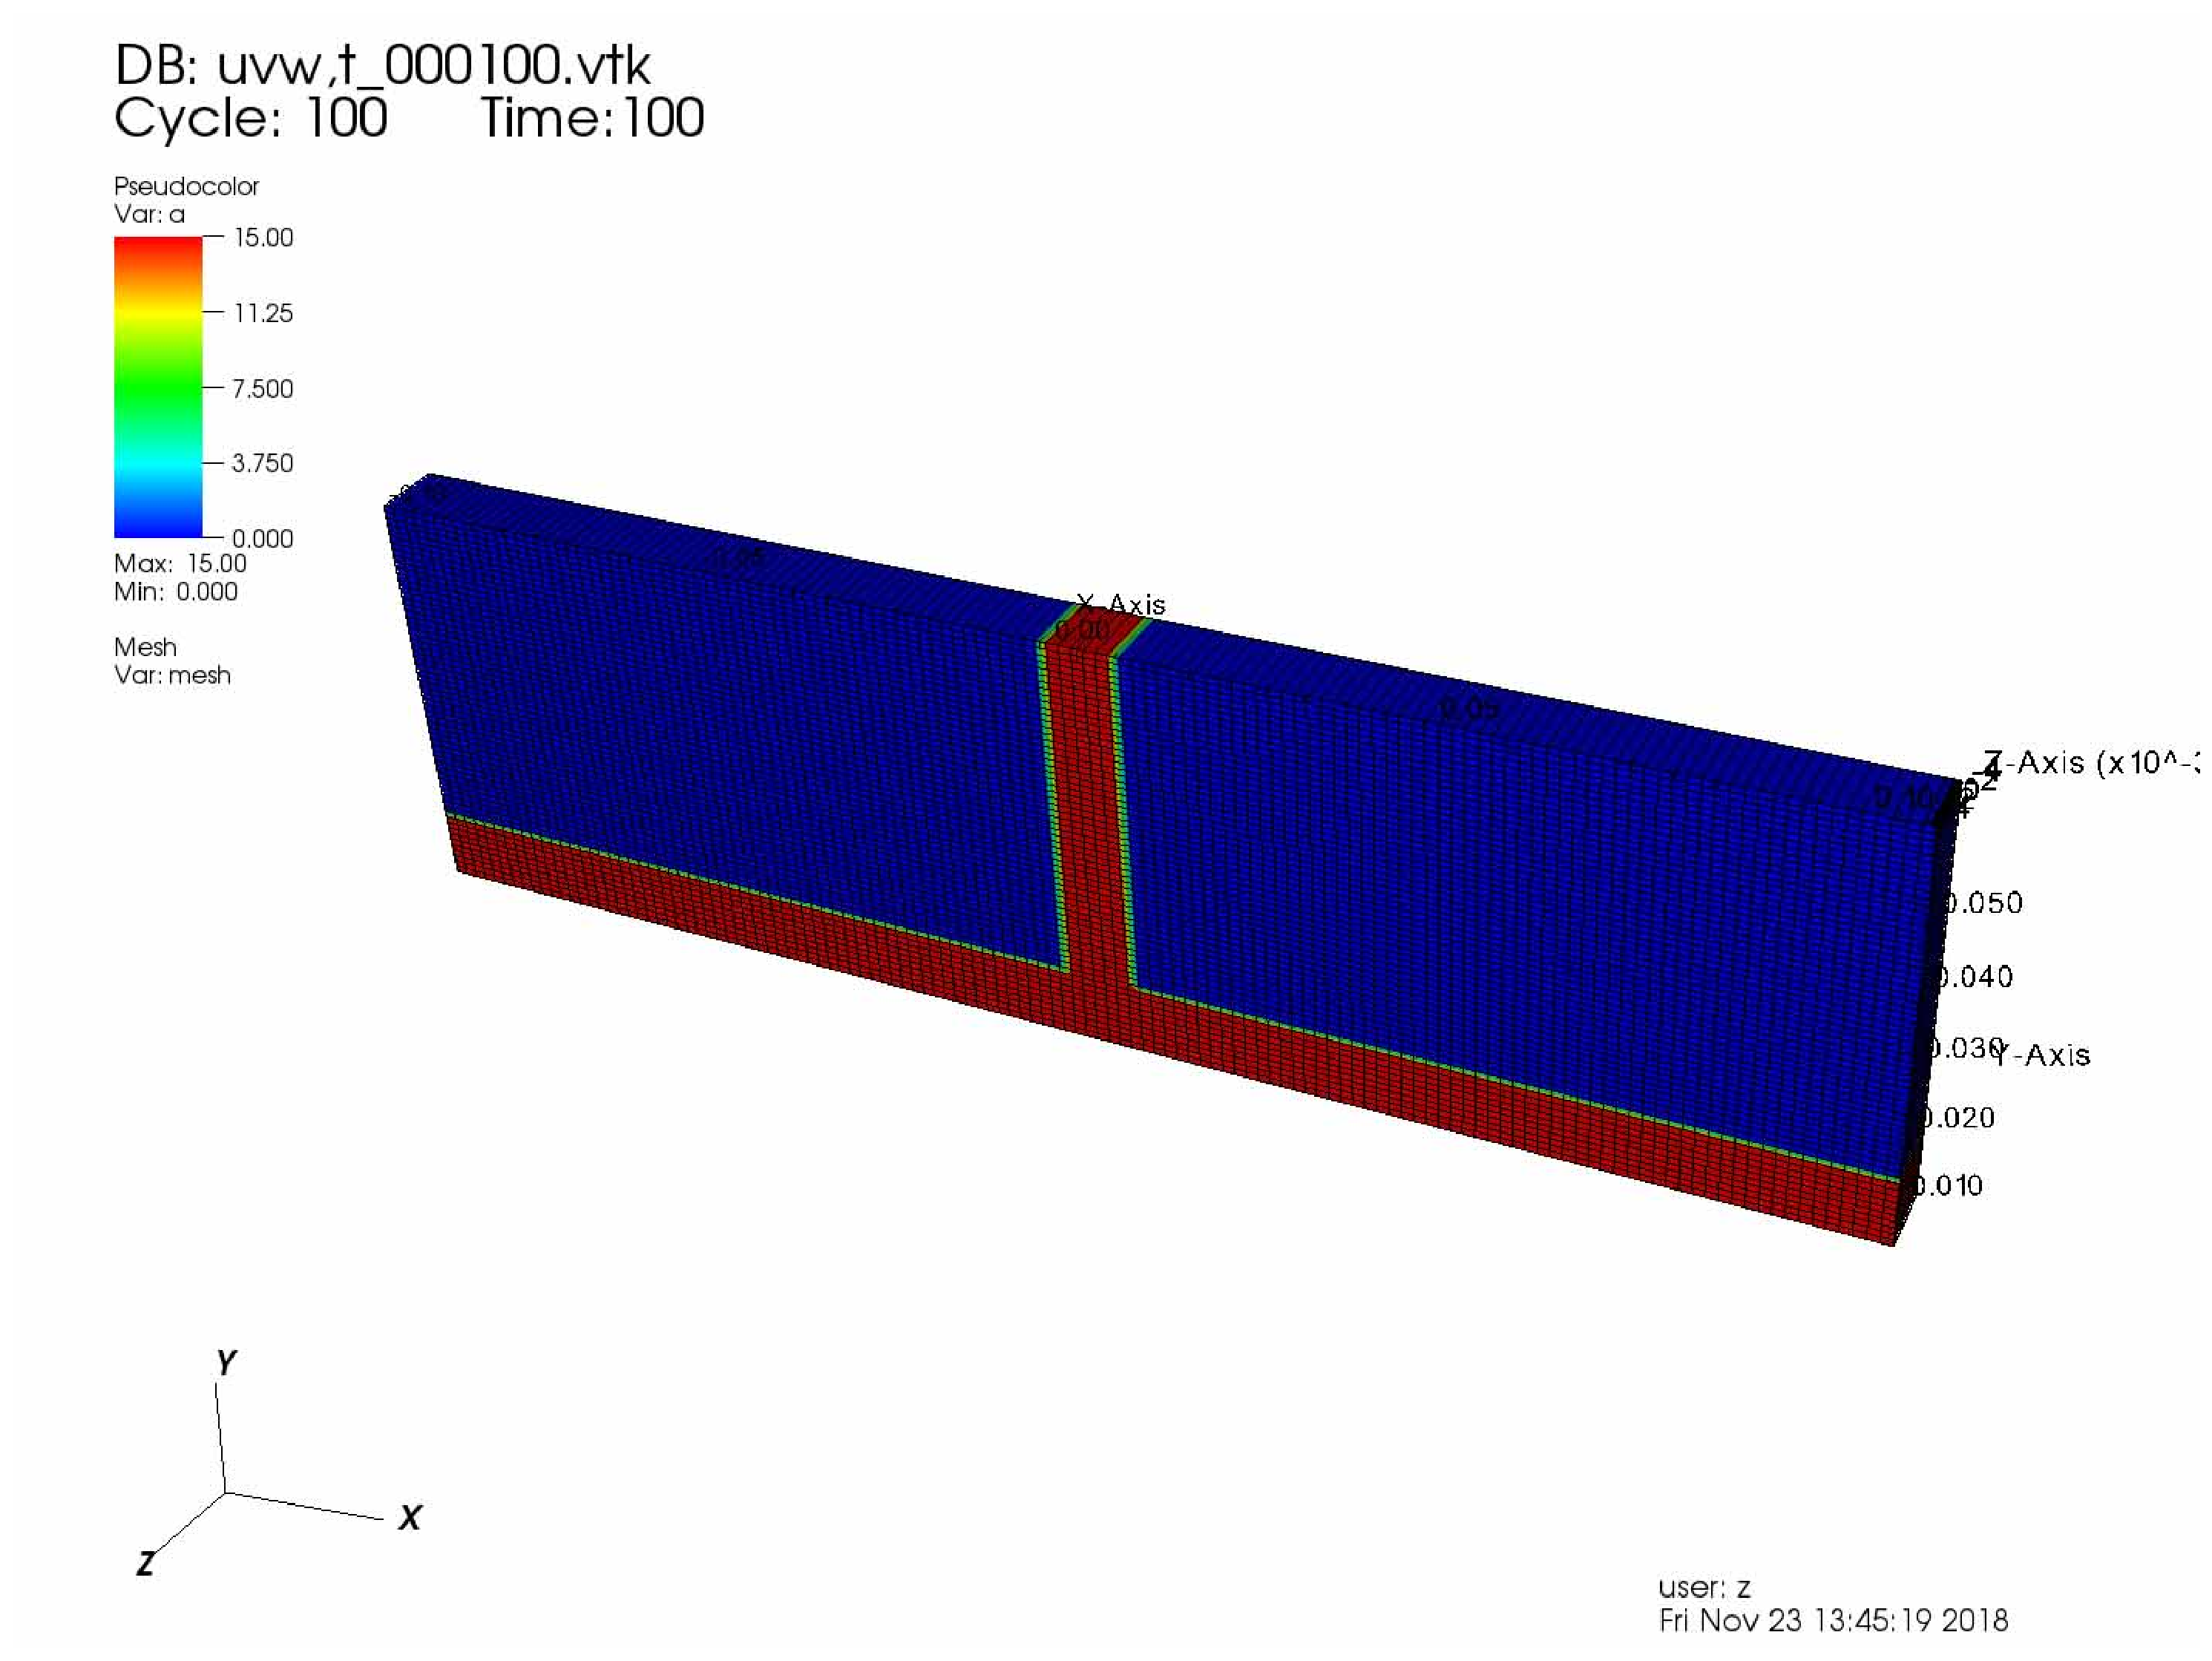
\includegraphics[scale=0.20]{Figures/10-LPT/10-03-physical-model-and-mesh.eps}}
    \put( 0, 0){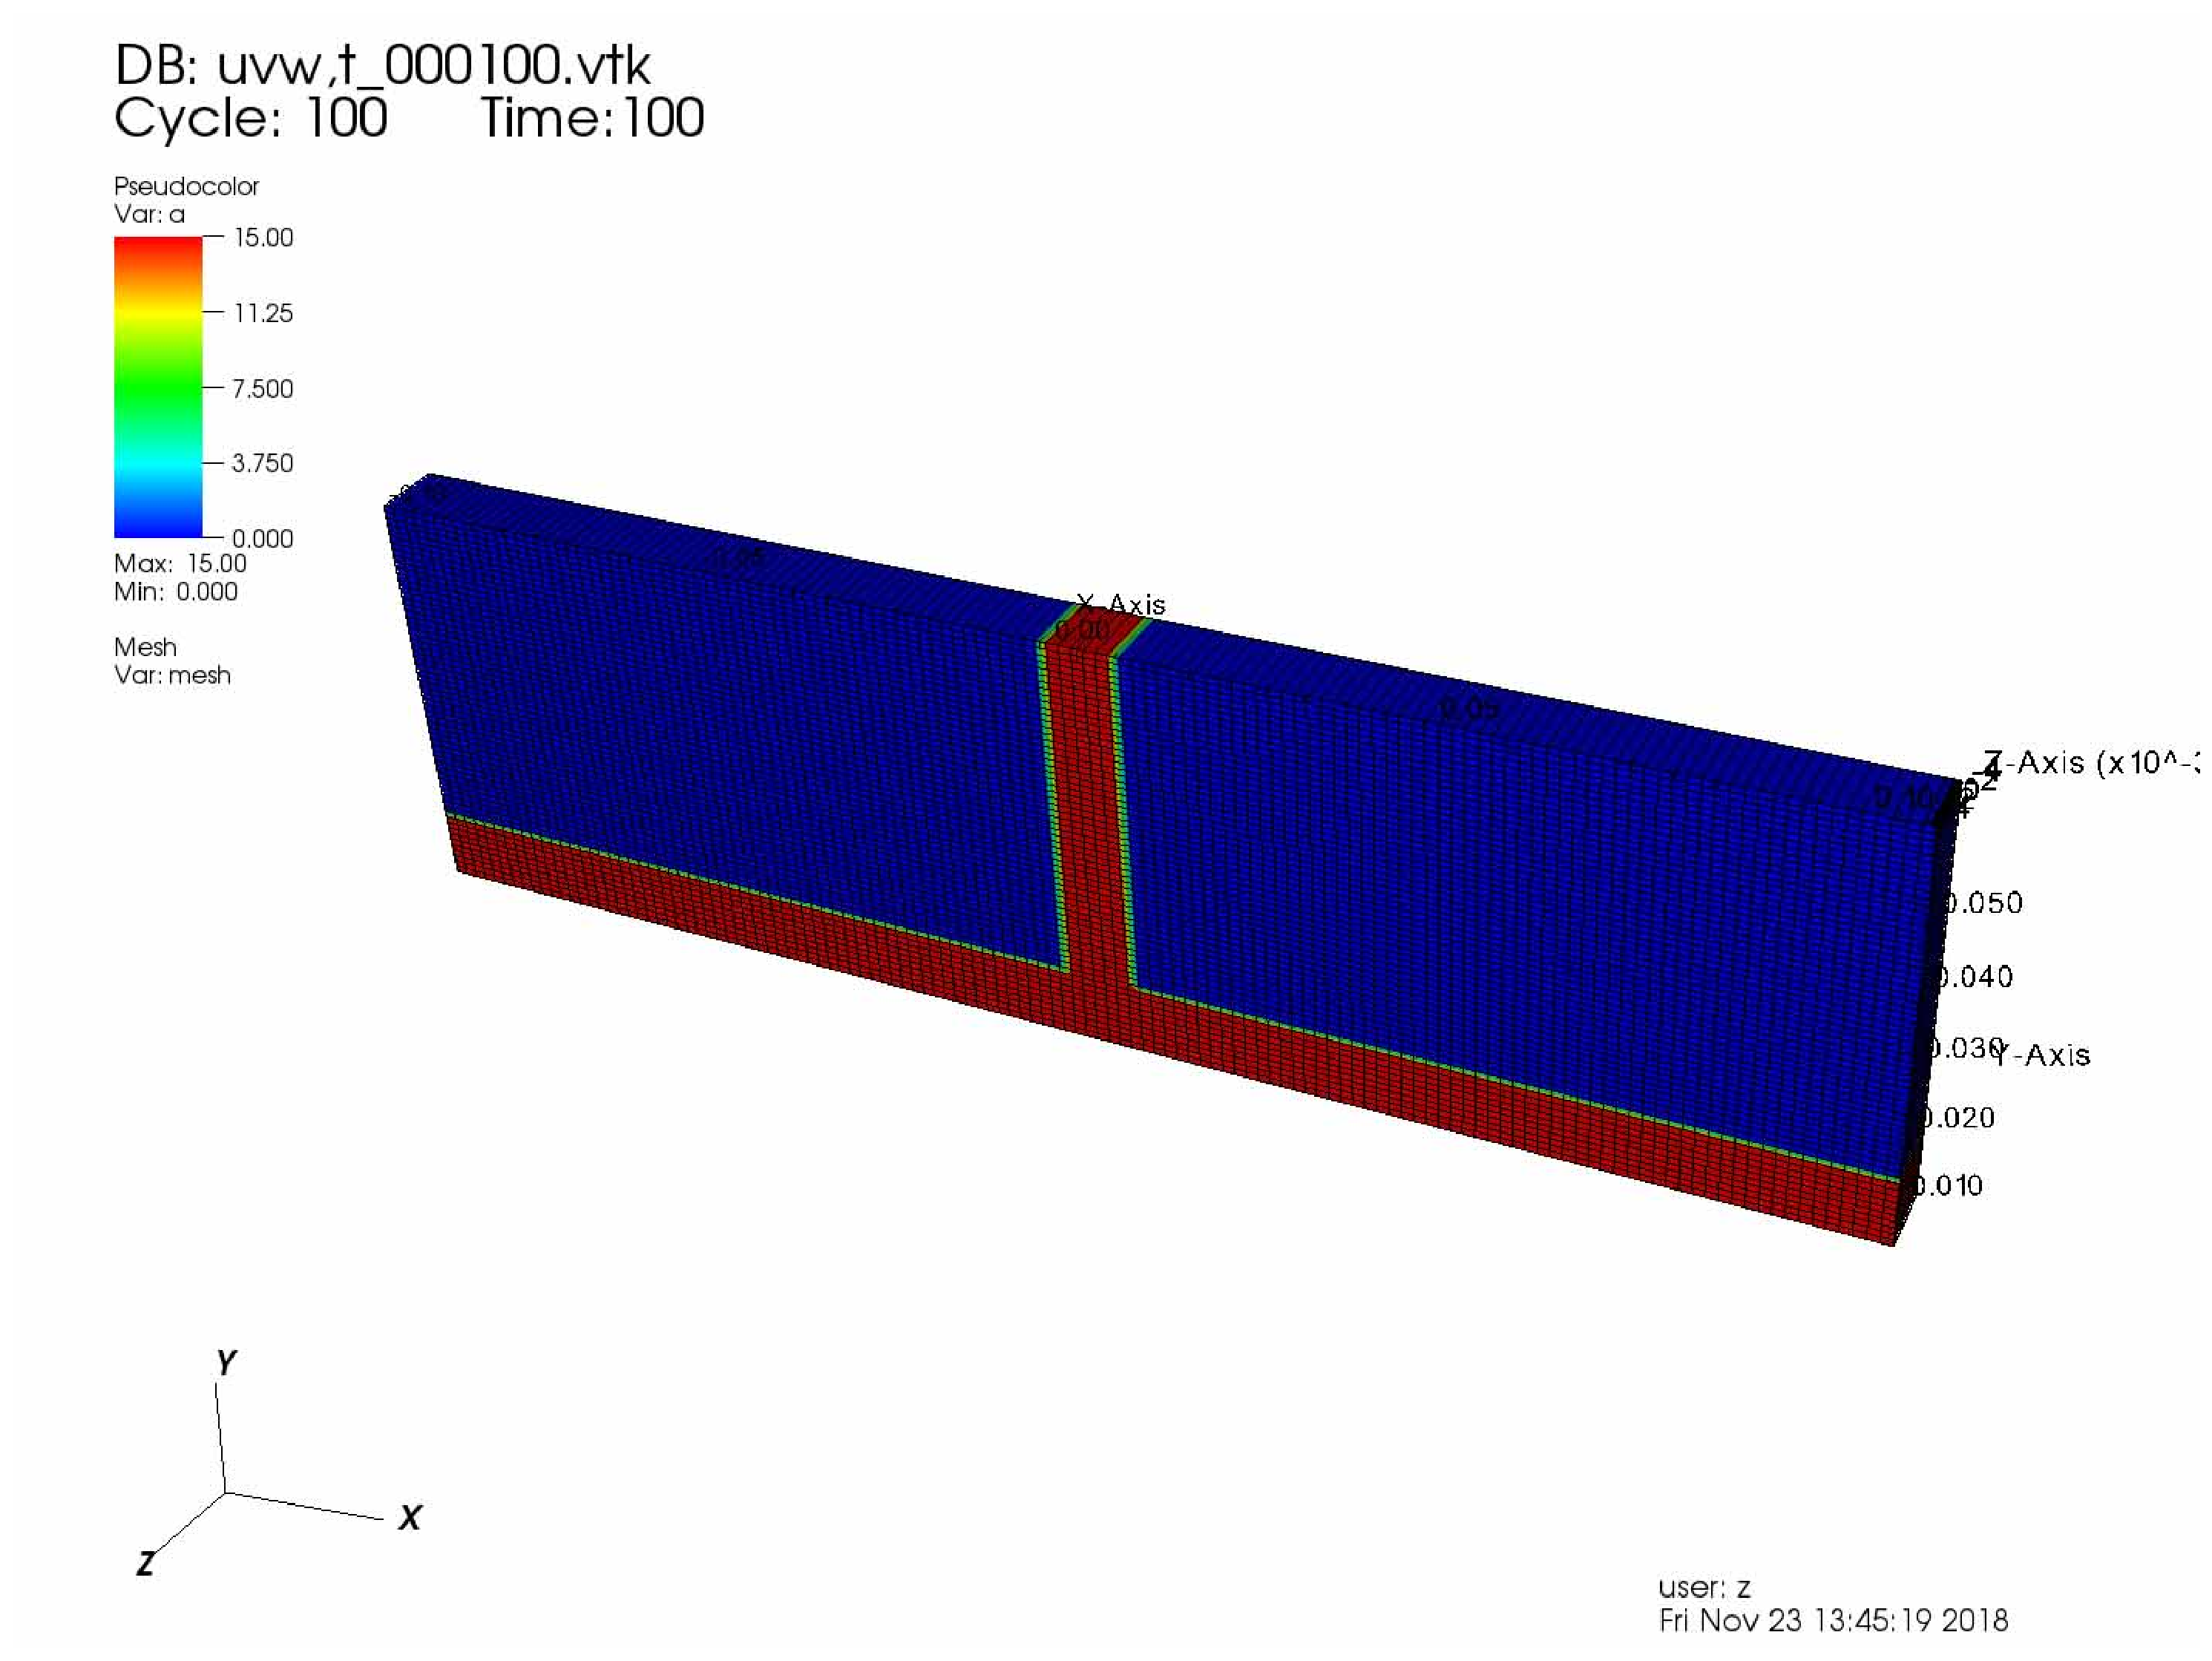
\includegraphics[width=70mm]{Figures/10-LPT/10-03-physical-model-and-mesh.eps}}
  \end{picture}
  \caption{Physical model and mesh for T-Junction.}
  \label{fig_tjpa}
\end{figure}

%-----------------------------%
%                             %
%  SinglePhase VelocityField  %
%                             %
%-----------------------------%
\begin{figure}[ht]
  \centering
  \setlength{\unitlength}{ 1mm}
  \begin{picture}( 90, 60)( 0, 0)
    \thickbox{ 90}{ 60}
    \put( 5, 0){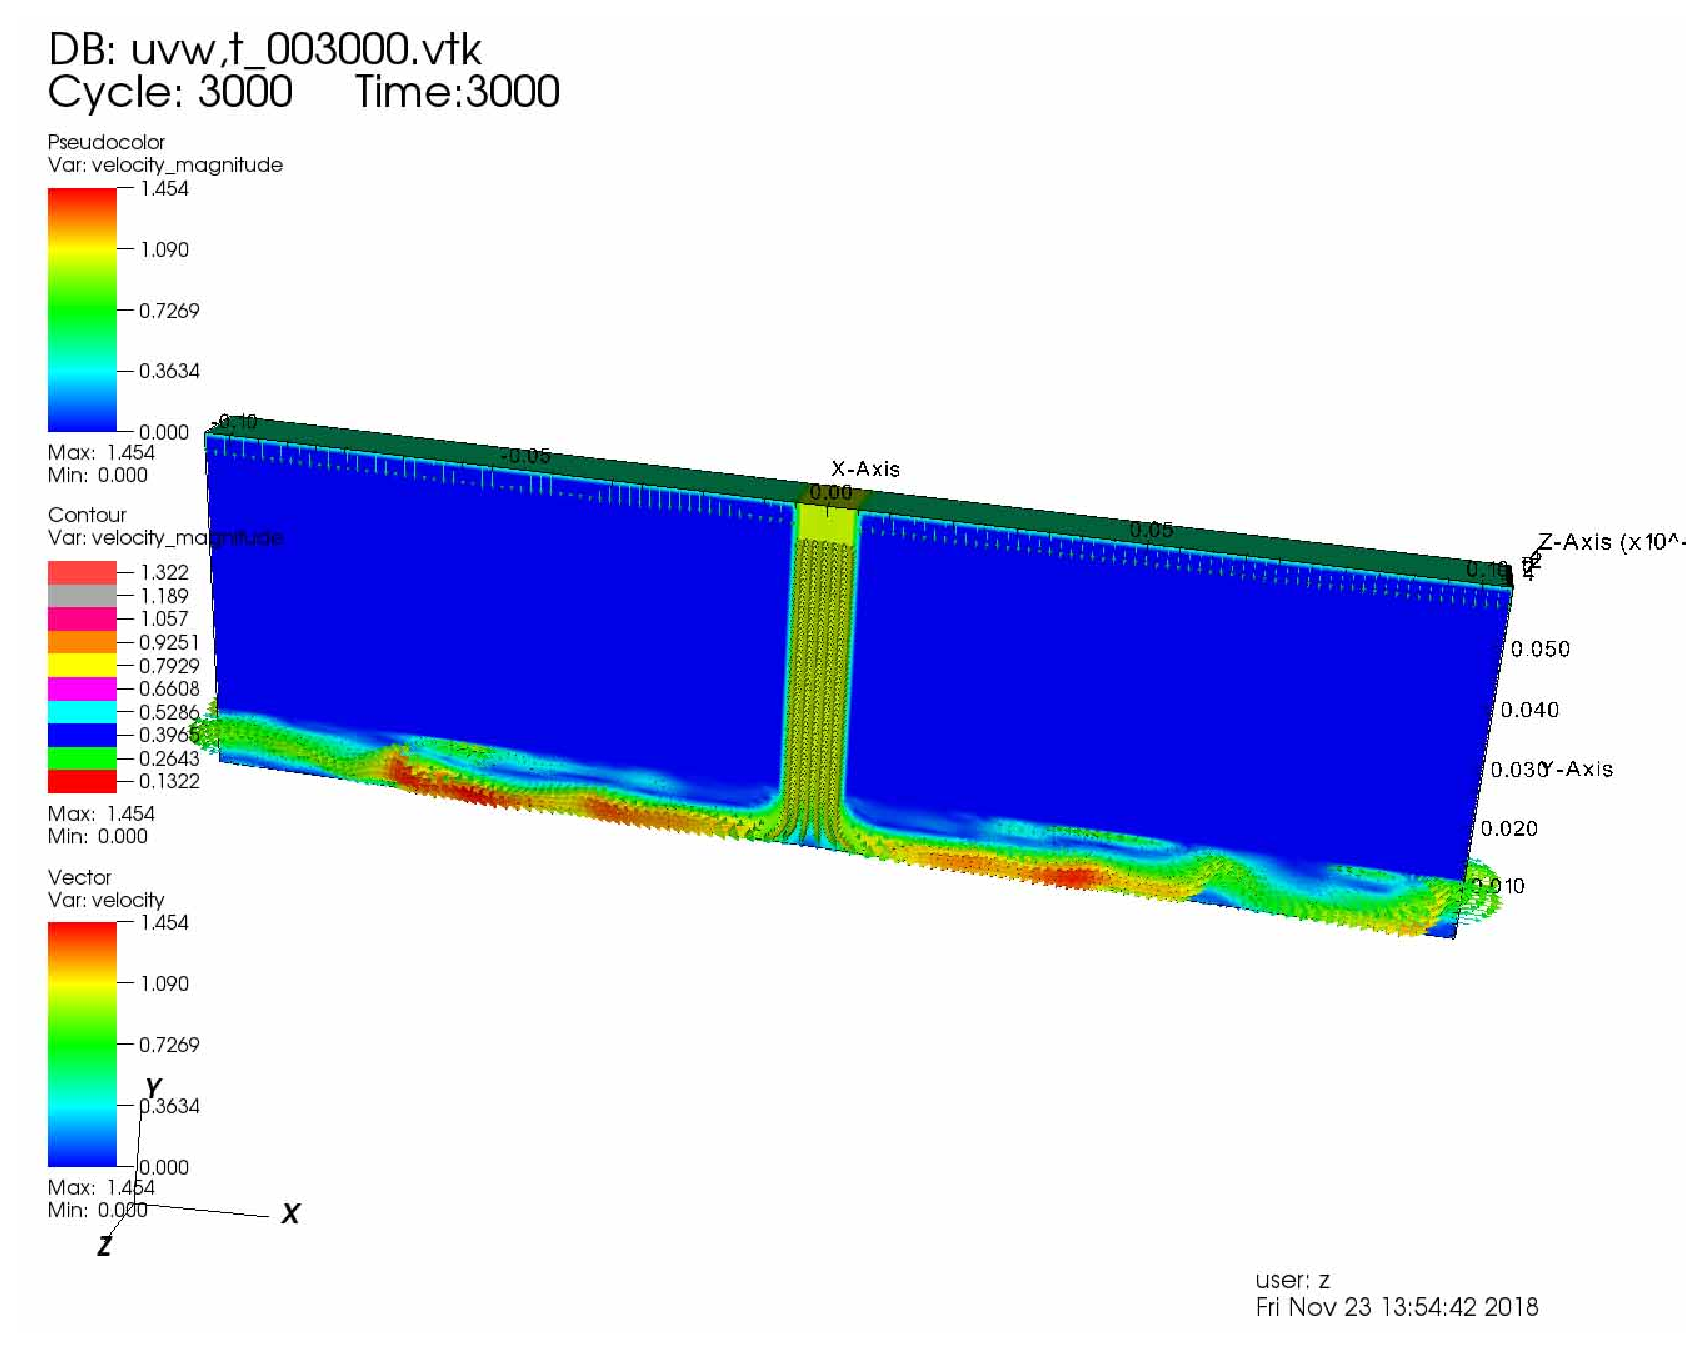
\includegraphics[width=80mm]{Figures/10-LPT/10-04-single-phase-velocity-field.eps}}
  \end{picture}
  \caption{Single phase velocity field in T-Junction.}
  \label{fig_tjpb}
\end{figure}

%-------------------------------%
%                               %
%  TwoPhase ParticleTrajectory  %
%                               %
%-------------------------------%
\begin{figure}[ht]
  \centering
  \setlength{\unitlength}{ 1mm}
  \begin{picture}( 100, 40)( 0, 0)
    \thickbox{ 100}{ 40}
    \put( 20, 0){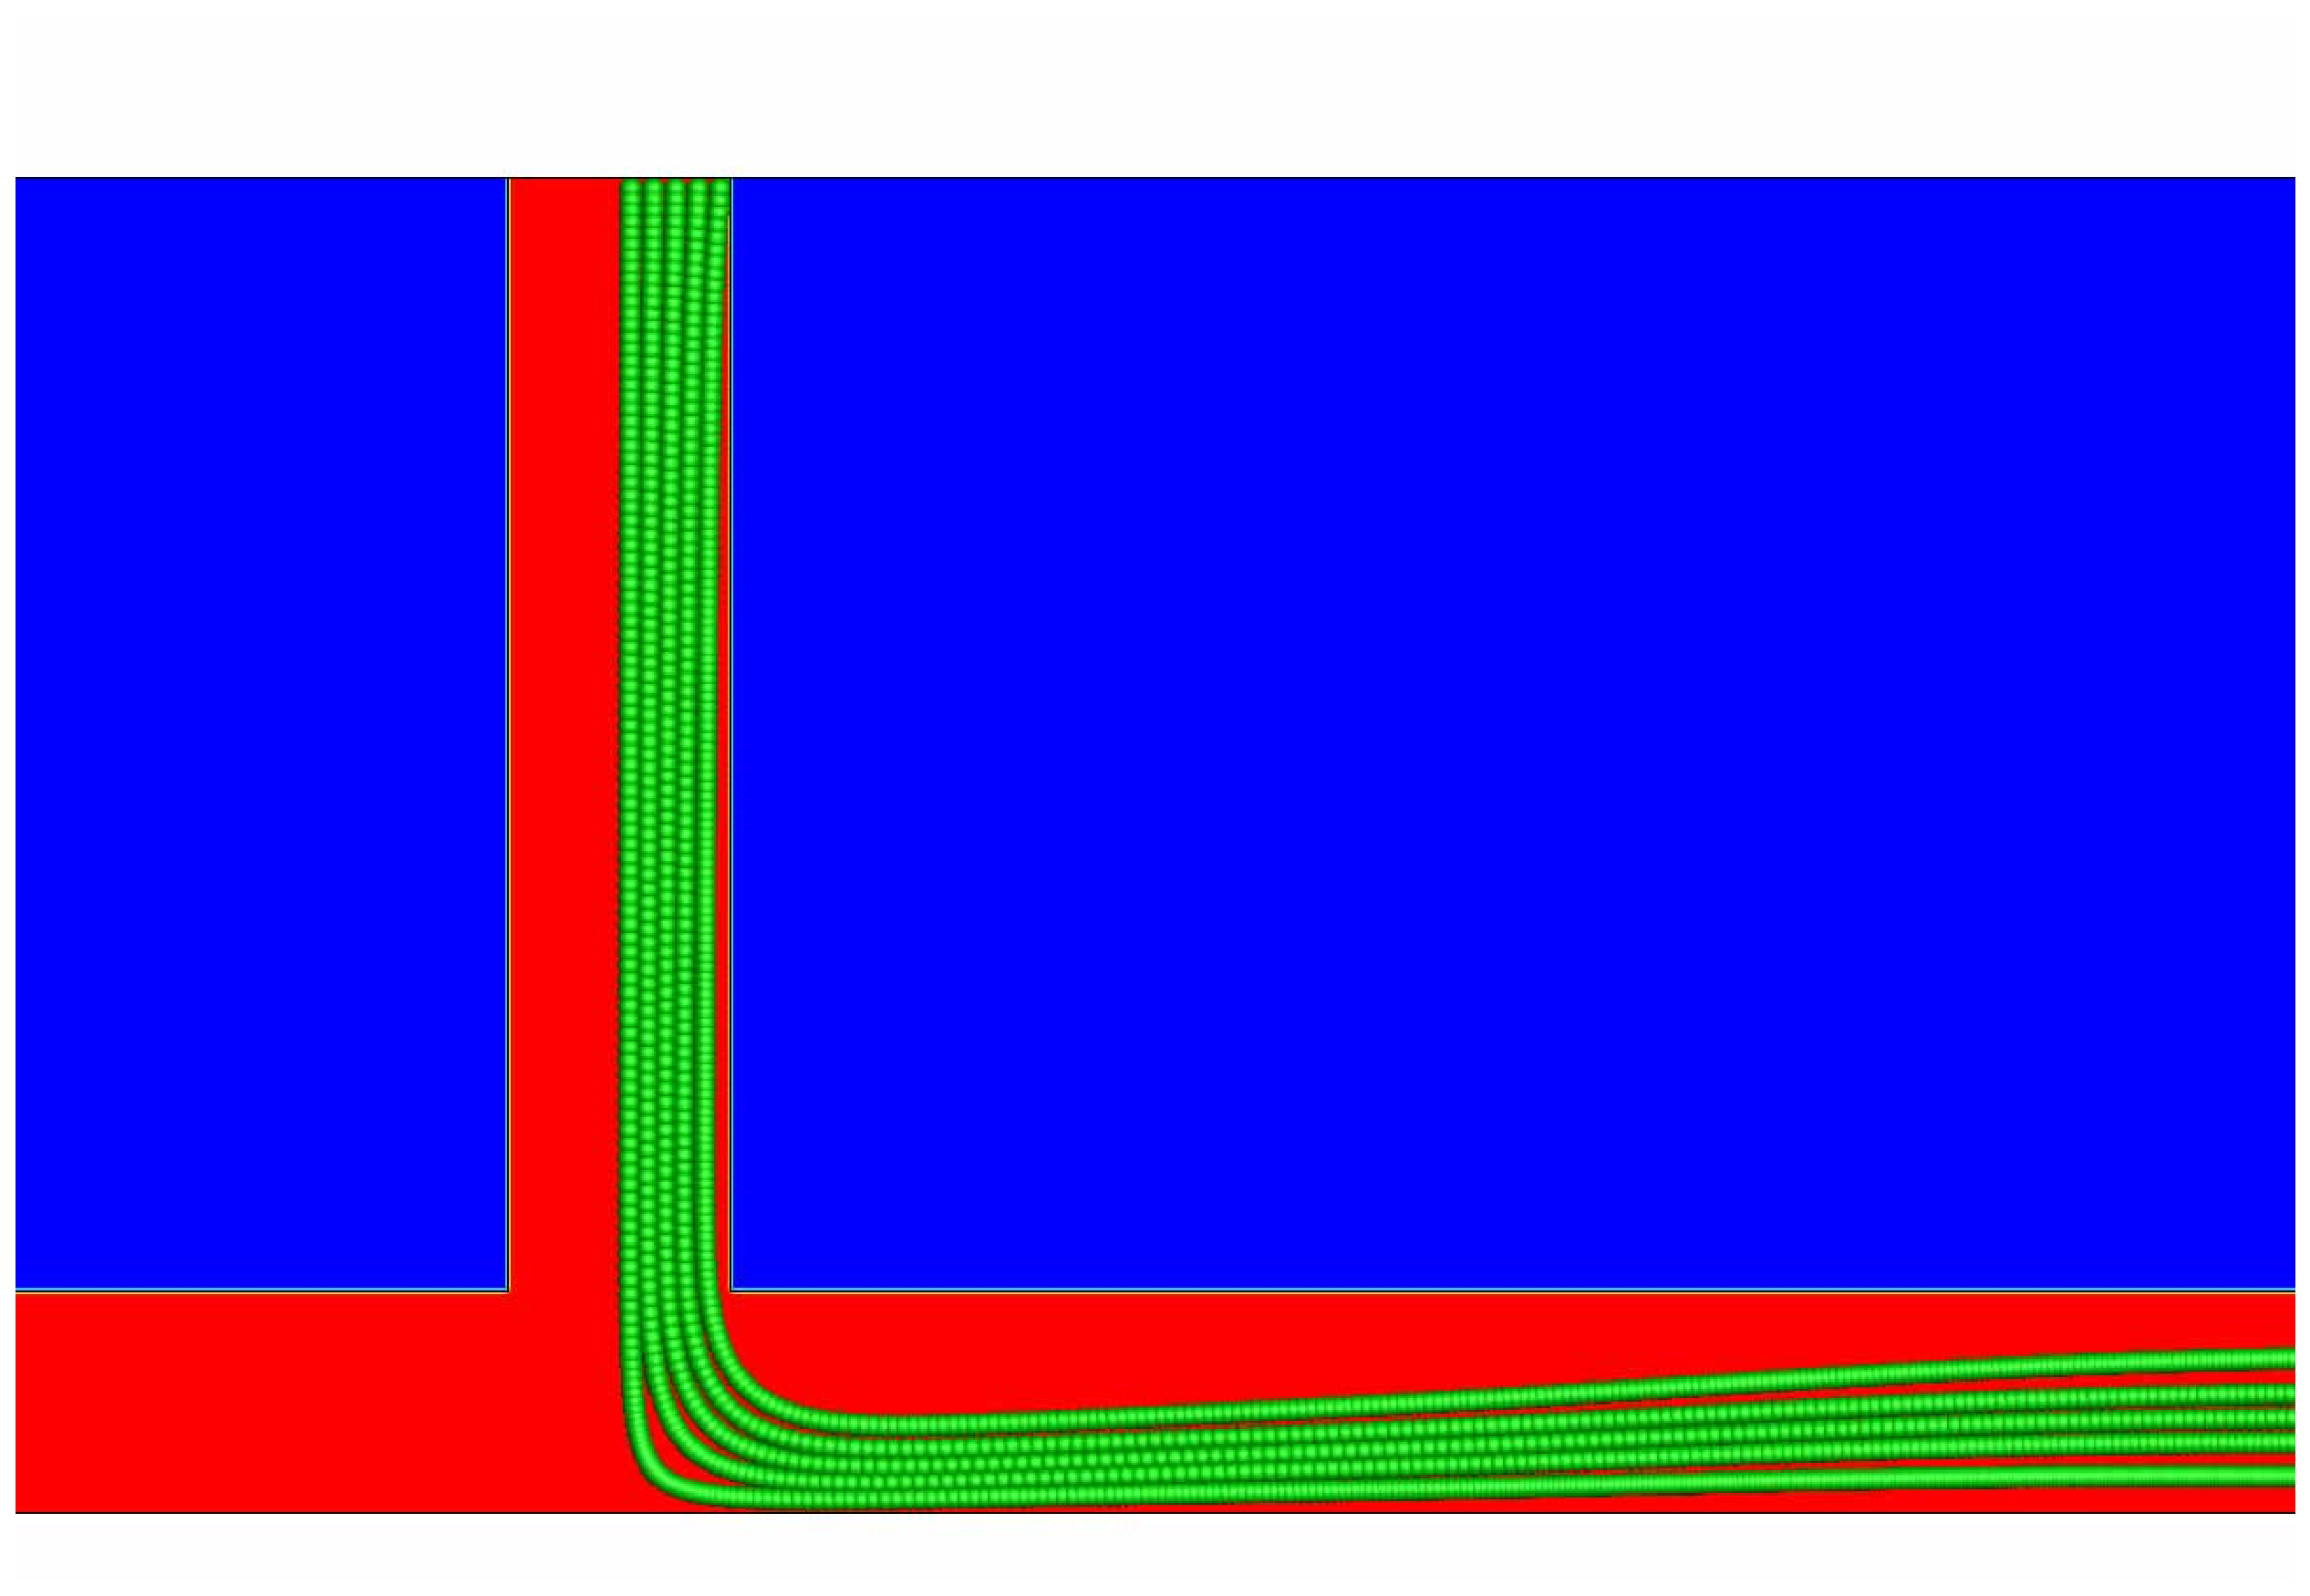
\includegraphics[scale=0.15]{Figures/10-LPT/10-05-two-phase-particle-trajectory.eps}}
  \end{picture}
  \caption{Particle trajectory in T-Junction.}
  \label{fig_tjpc}
\end{figure}

%-----------------------------------%
%                                   %
%  TwoPhase TrajectoryVerification  %
%                                   %
%-----------------------------------%
\begin{figure}[ht]
  \centering
  \setlength{\unitlength}{ 1mm}
  \begin{picture}( 150, 50)( 0, 0)
    \thickbox{ 150}{ 50}
    \put( 10, 0){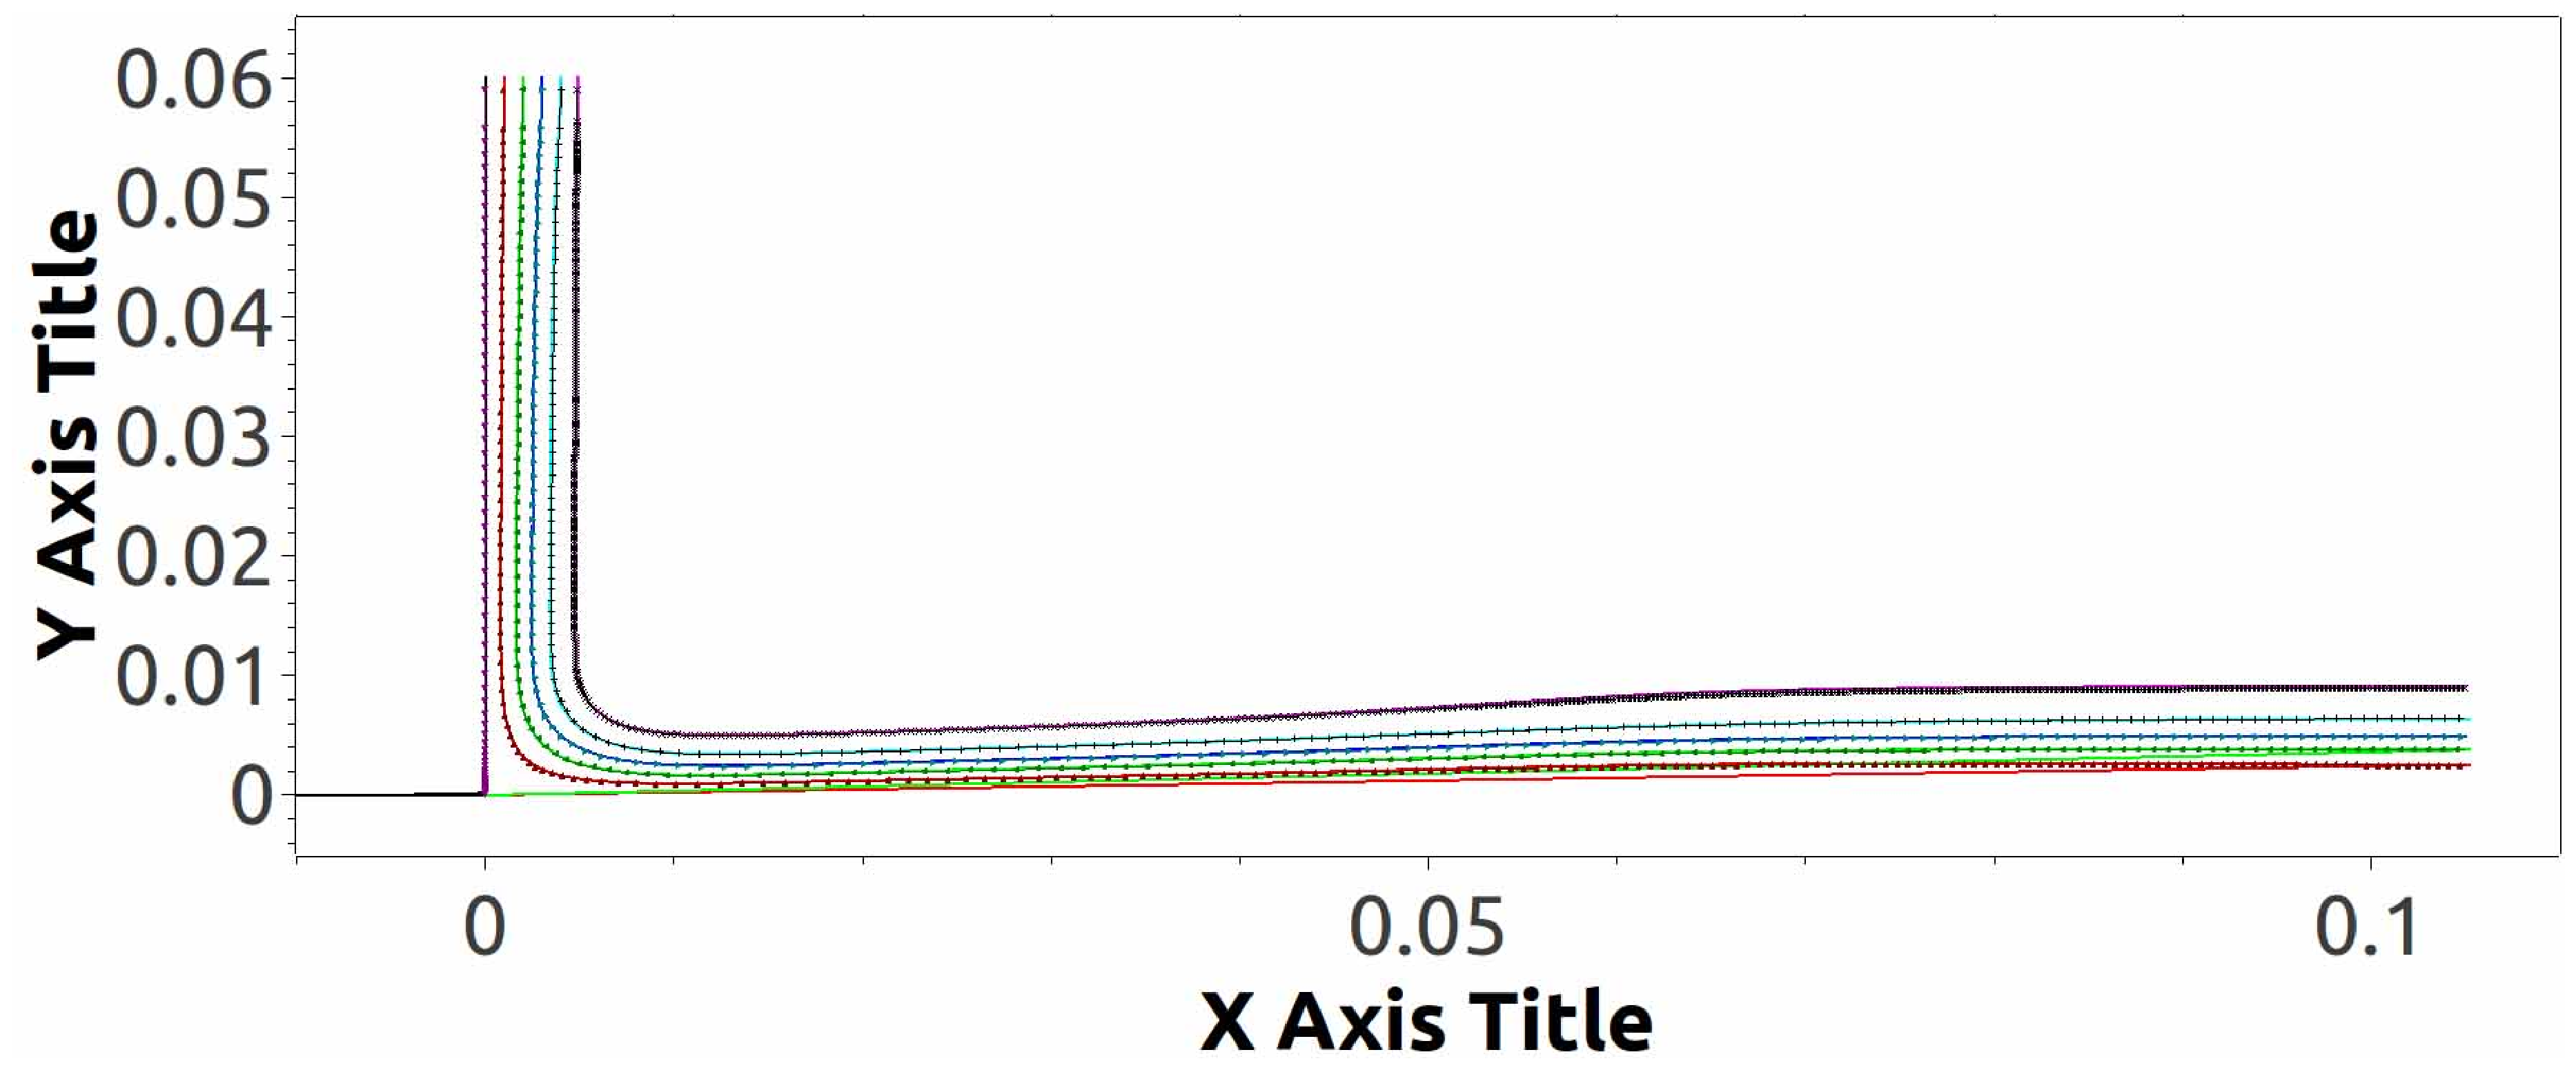
\includegraphics[scale=0.20]{Figures/10-LPT/10-06-two-phase-trajectory-verification.eps}}
  \end{picture}
  \caption{Particle trajectory verification.}
  \label{fig_tjpd}
\end{figure}

%---------------------------------%
%                                 %
%  TwoPhase TrajectoryValidation  %
%                                 %
%---------------------------------%
\begin{figure}[ht]
  \centering
  \setlength{\unitlength}{ 1mm}
  \begin{picture}( 120, 110)( 0, 0)
    \thickbox{ 120}{ 110}
    \put( 0, 0){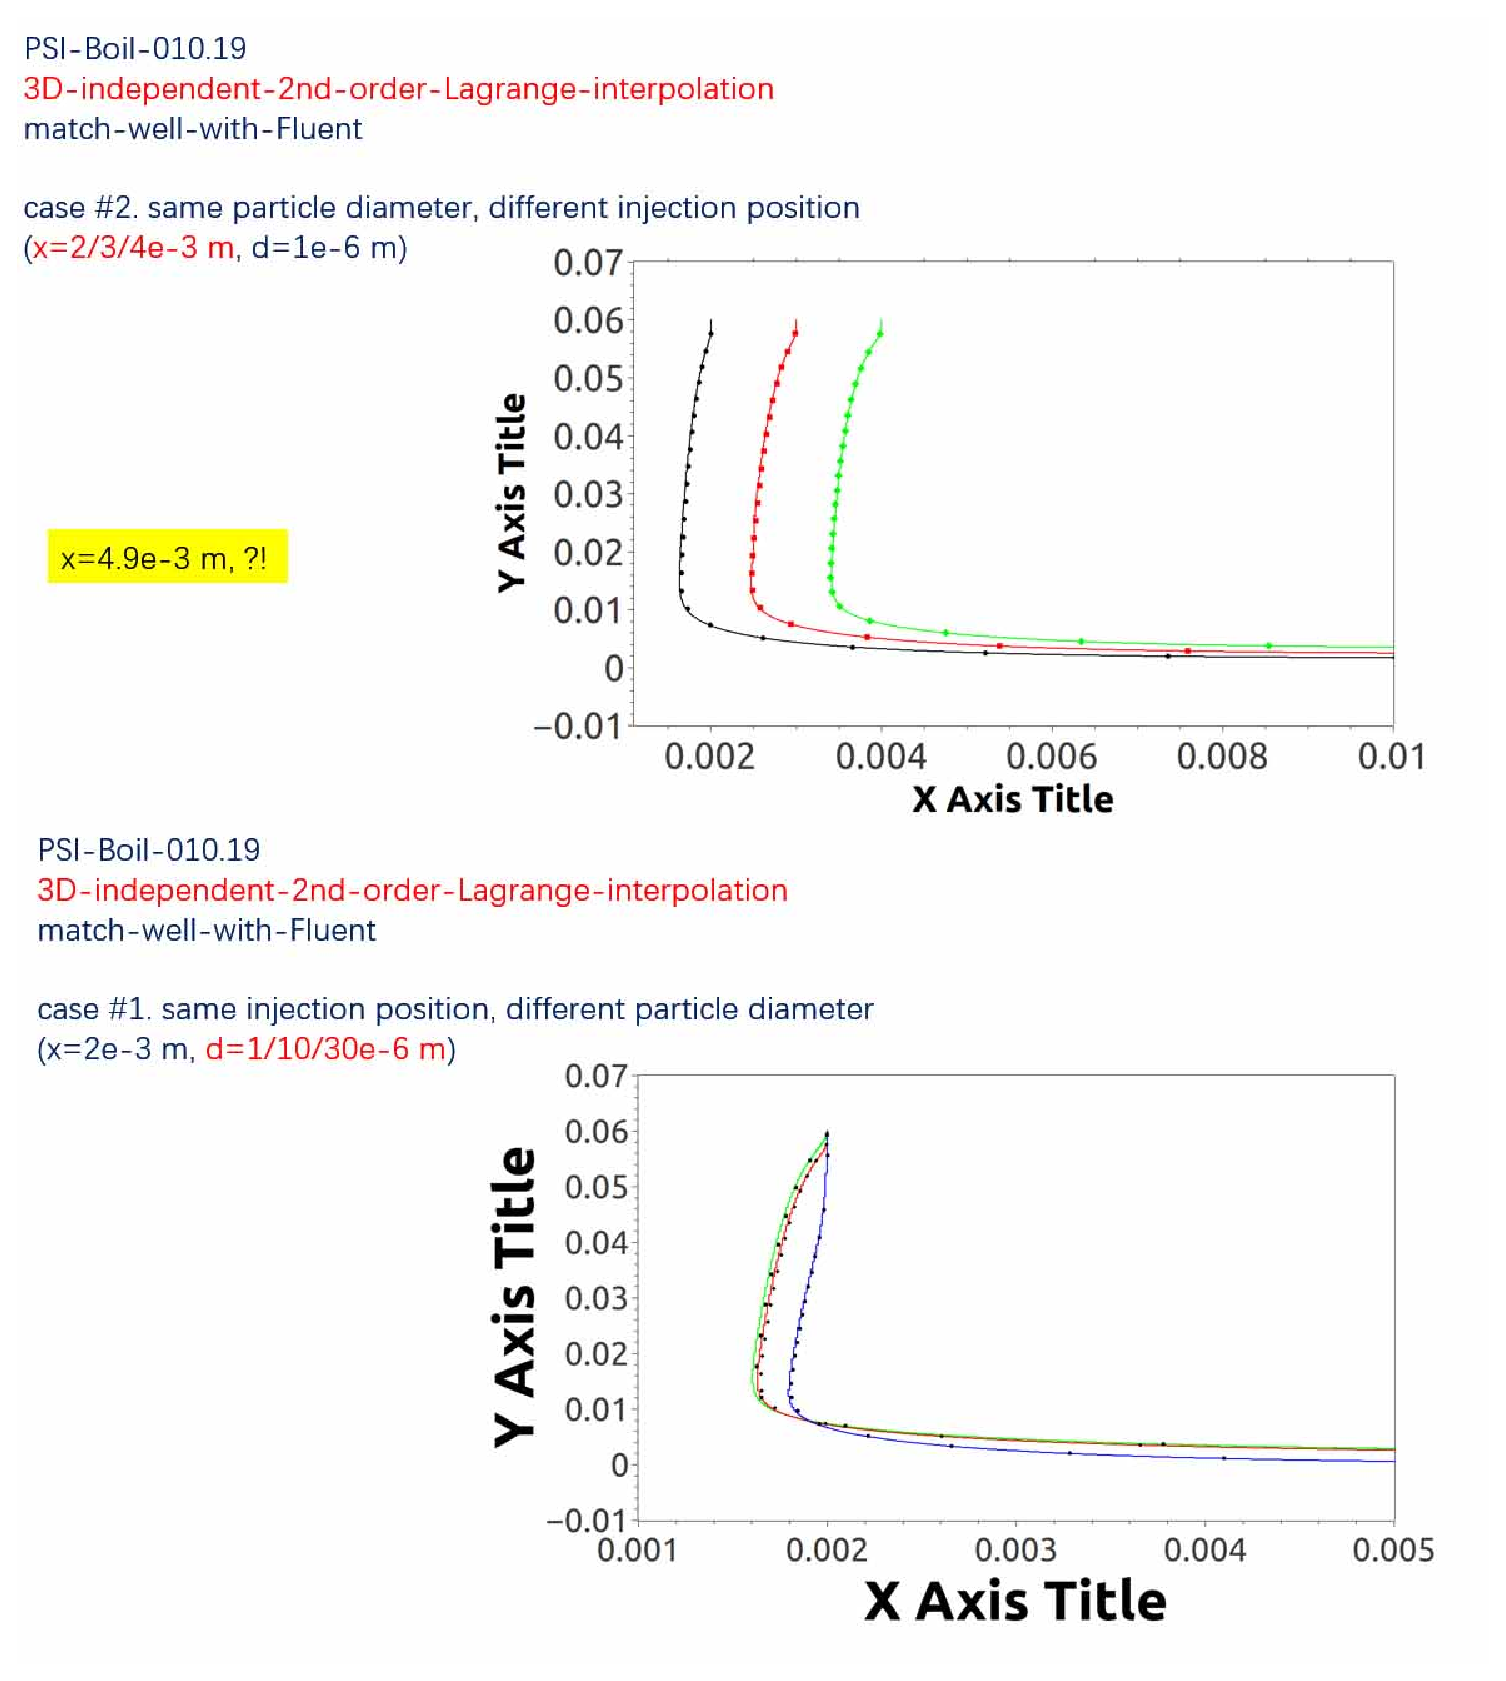
\includegraphics[scale=0.60]{Figures/10-LPT/10-07-two-phase-trajectory-validation.eps}}
  \end{picture}
  \caption{Particle trajectory validation.}
  \label{fig_tjpe}
\end{figure}


\clearpage
\subsection{One-dimensional particle deposition on dispersed surface}

%-----------------%
%                 %
%  1d-deposition  %
%                 %
%-----------------%
\begin{figure}[ht]
  \centering
  \setlength{\unitlength}{ 1mm}
  \begin{picture}( 250, 160)( 0, 0)
    \thickbox{ 250}{ 160}
    \put( -10, 0){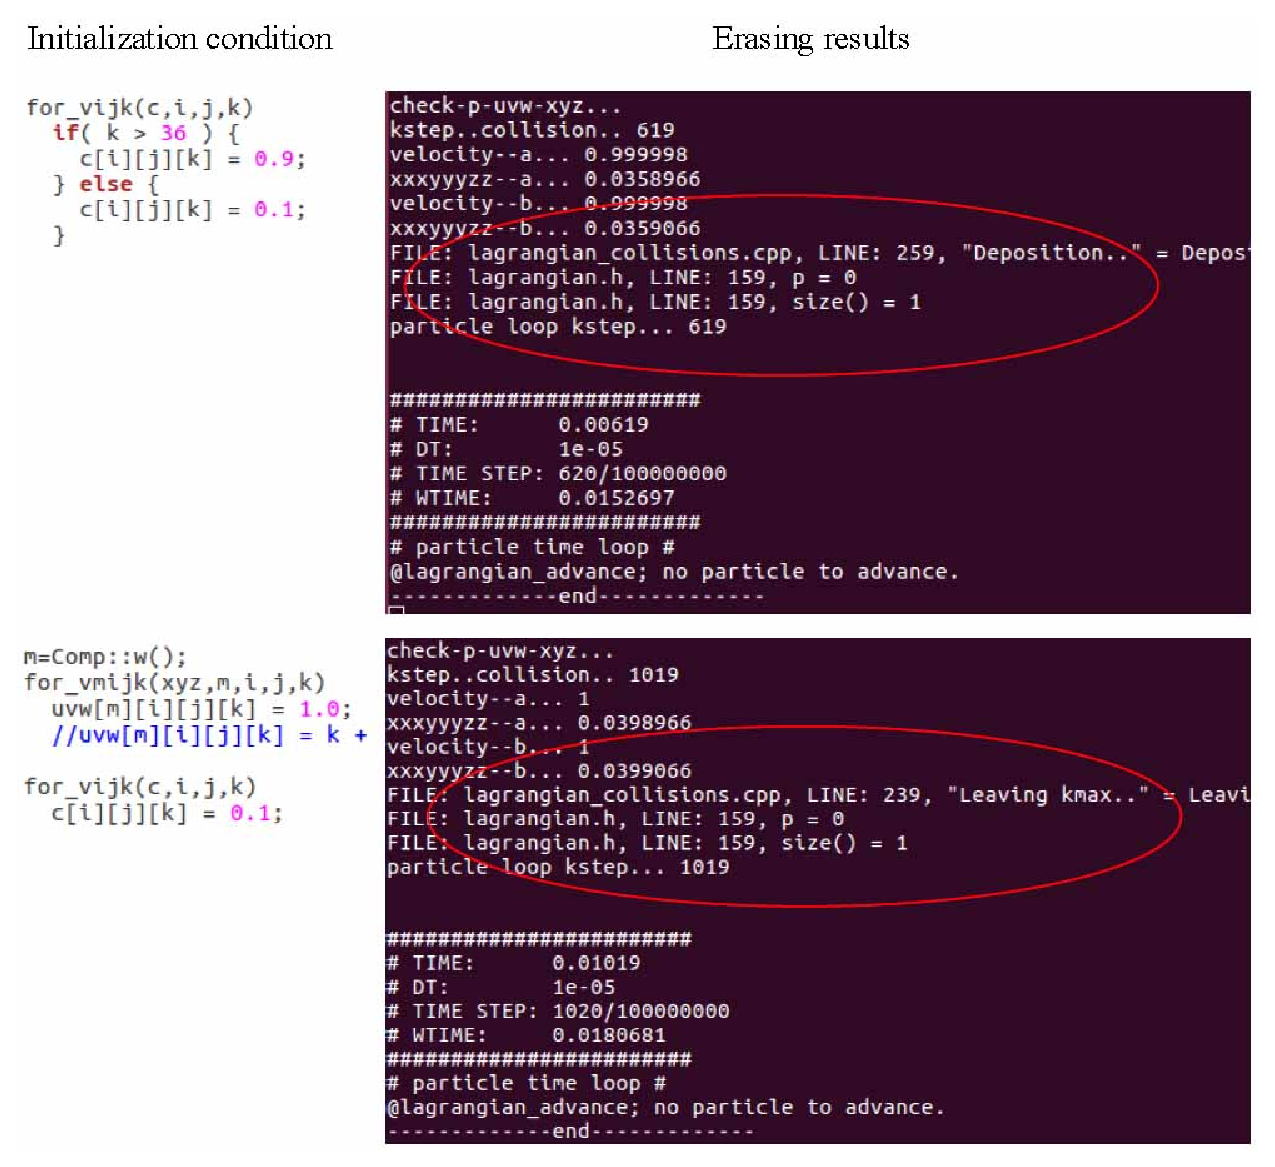
\includegraphics[scale=0.80]{Figures/10-LPT/10-08-1d-deposition.eps}}
  \end{picture}
  \caption{One-dimensional particle deposition on dispersed surface.}
  \label{fig_1dparticledepostion}
\end{figure}


\clearpage
\subsection{Terminal velocity verification}

%-----------------%
%                 %
%  1d-particlevp  %
%                 %
%-----------------%
\begin{figure}[ht]
  \centering
  \setlength{\unitlength}{ 1mm}
  \begin{picture}(160, 110)( 0, 0)
    \thickbox{160}{ 110}
    \put( 20, 0){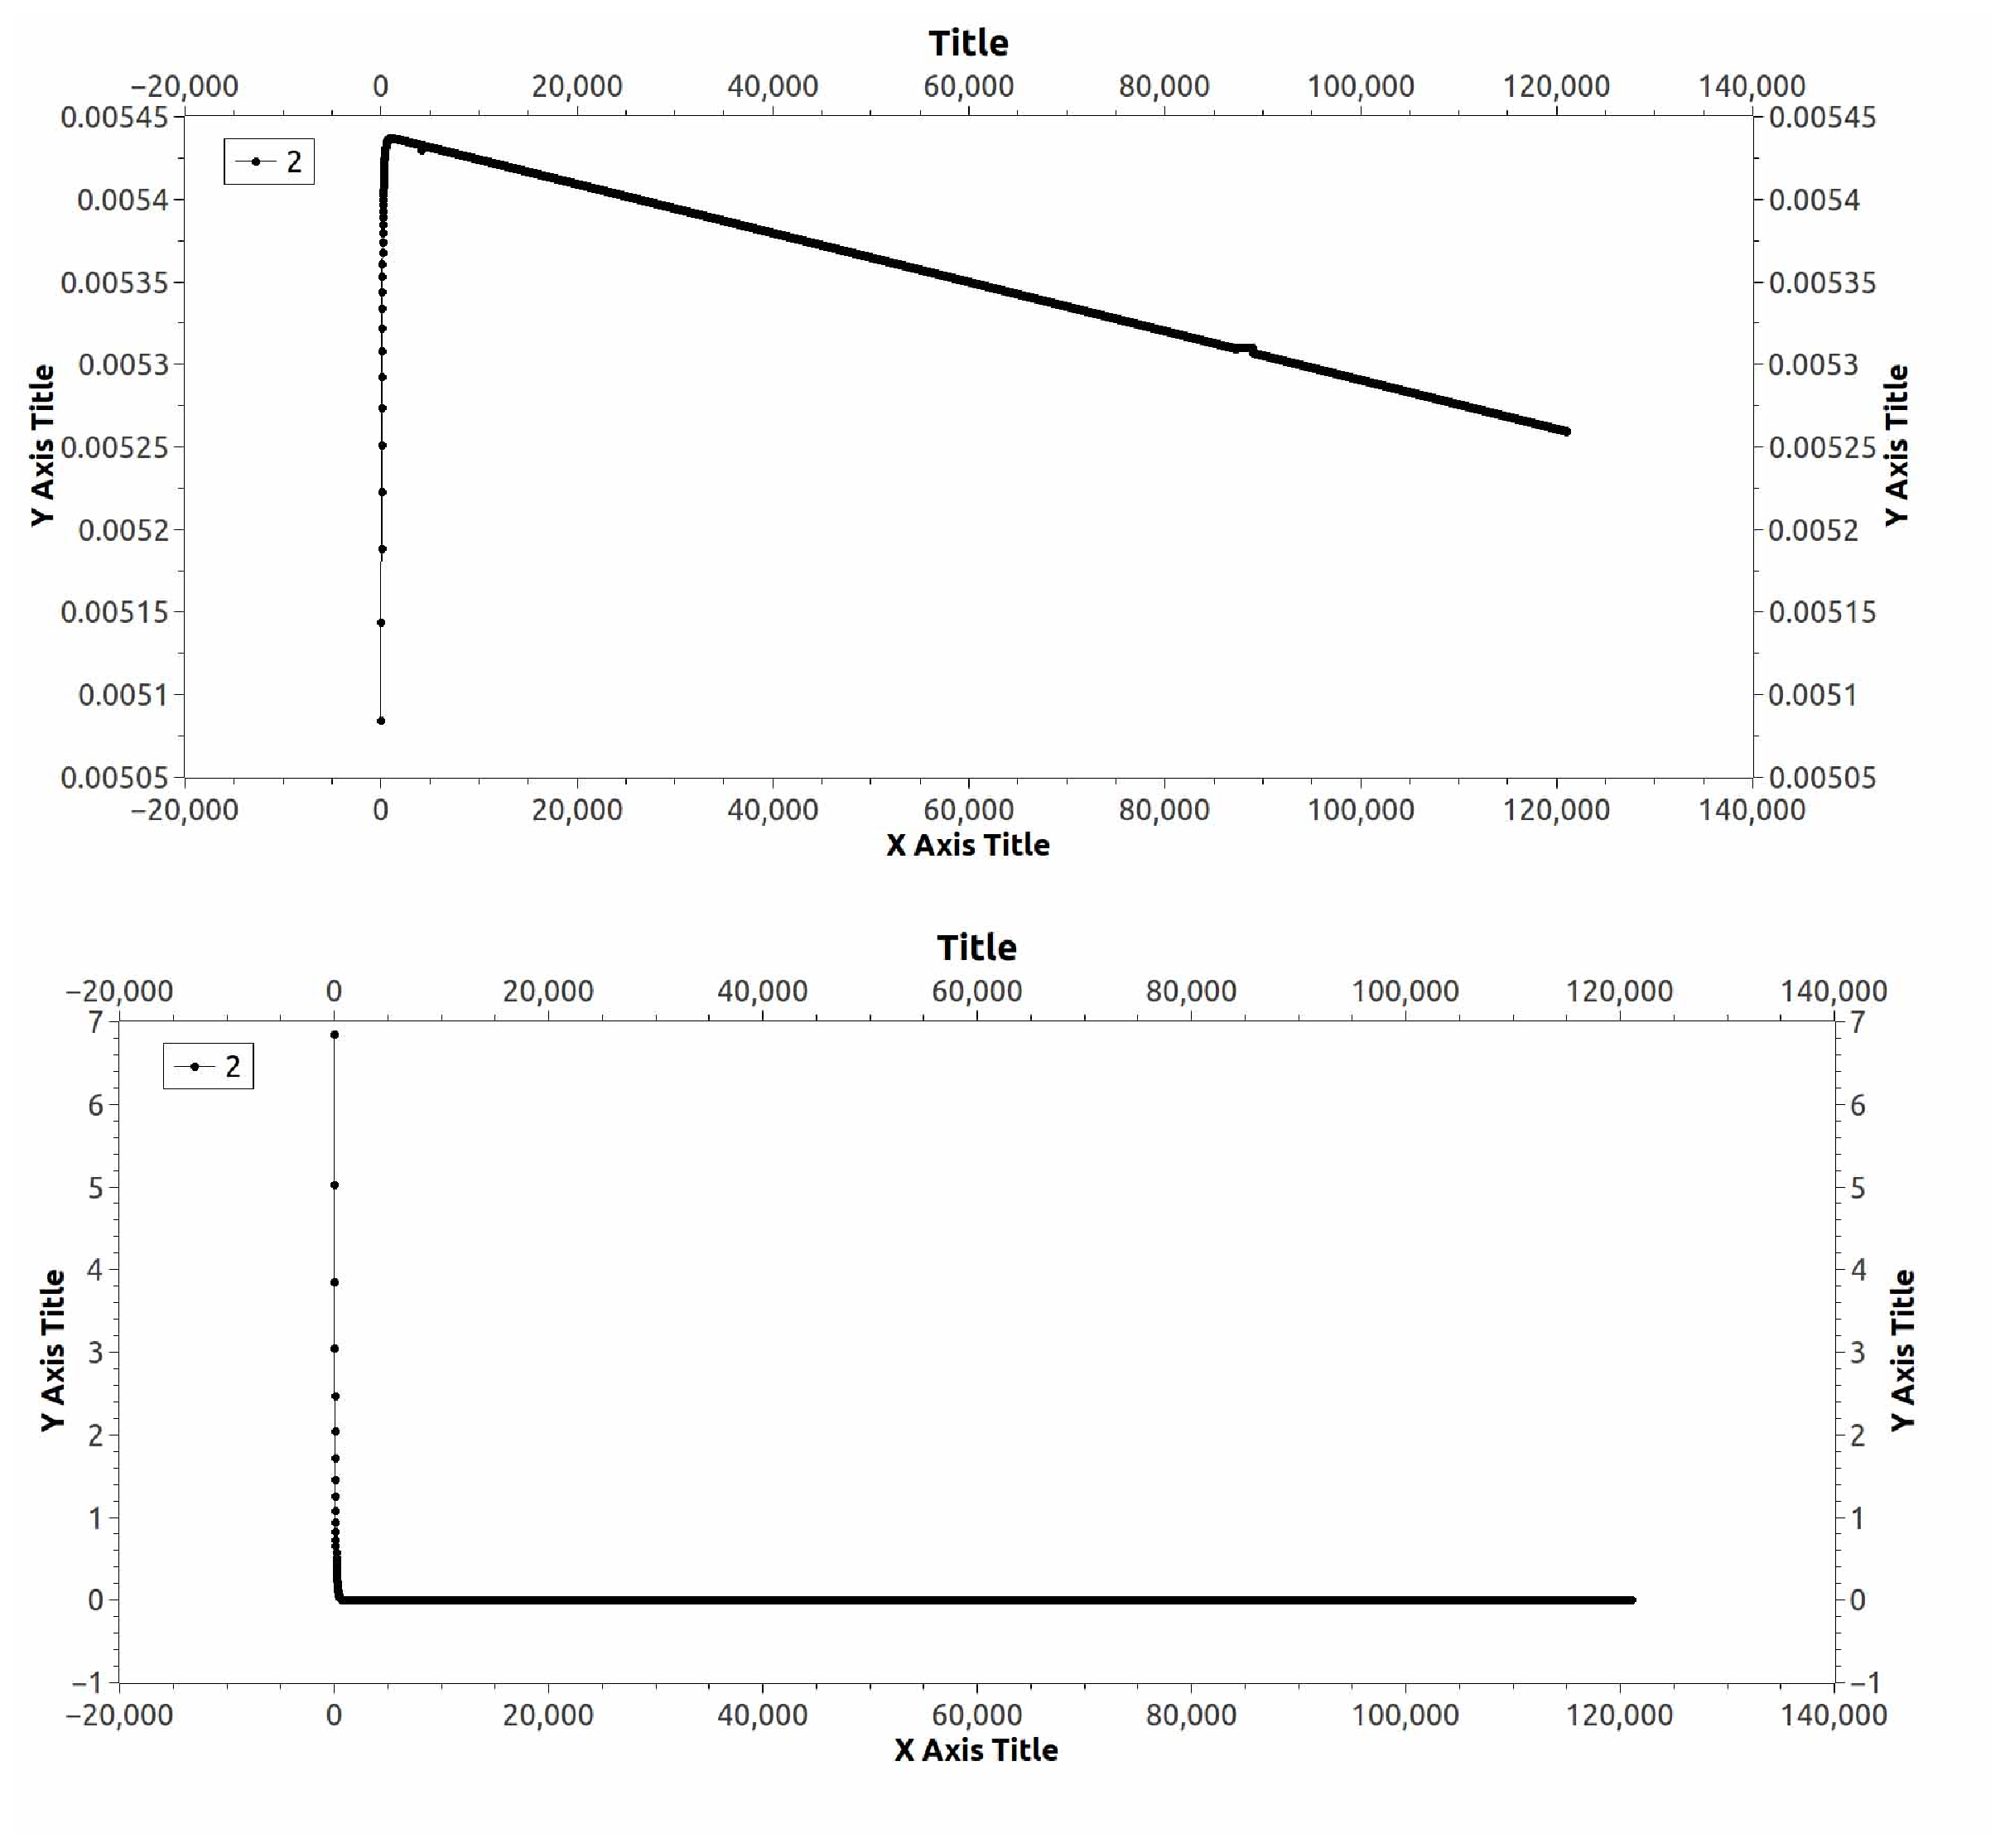
\includegraphics[scale=0.30]{Figures/10-LPT/10-09-velocity-and-position.eps}}
  \end{picture}
  \caption{The change of particle velocity and position.}
  \label{fig_1dparticlevp}
\end{figure}

%--------------------------------%
%                                %
%  terminal velocity difference  %
%                                %
%--------------------------------%
\begin{figure}[ht]
  \centering
  \setlength{\unitlength}{ 1mm}
  \begin{picture}( 190, 40)( 0, 0)
    \thickbox{ 190}{ 40}
    \put( -20, 0){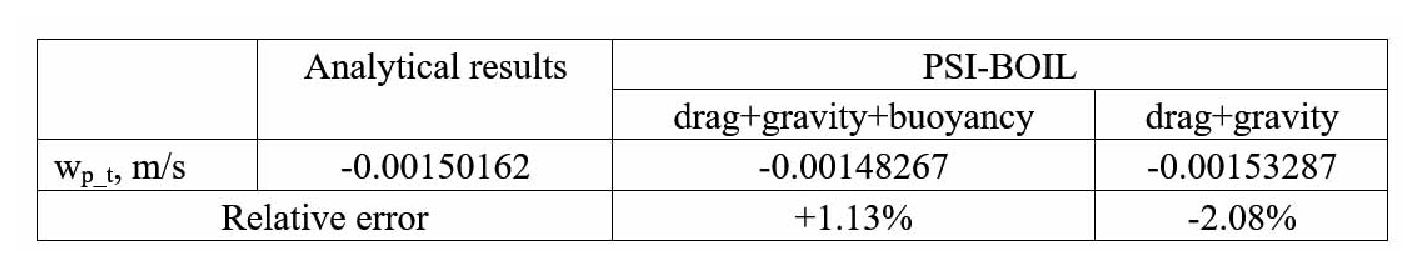
\includegraphics[scale=0.80]{Figures/10-LPT/10-10-terminal-velocity-difference.eps}}
  \end{picture}
  \caption{Difference between analytical and numerical results.}
  \label{fig_1dterminalvelocitydifference}
\end{figure}


\clearpage
\subsection{Particle deposition of multiphase flow}

%-----------------------------%
%                             %
%  SinglePhase Velocityfield  %
%                             %
%-----------------------------%
\begin{figure}[ht]
  \centering
  \setlength{\unitlength}{ 1mm}
  \begin{picture}( 60, 100)( 0, 0)
    \thickbox{ 60}{ 100}
    \put( -10, 0){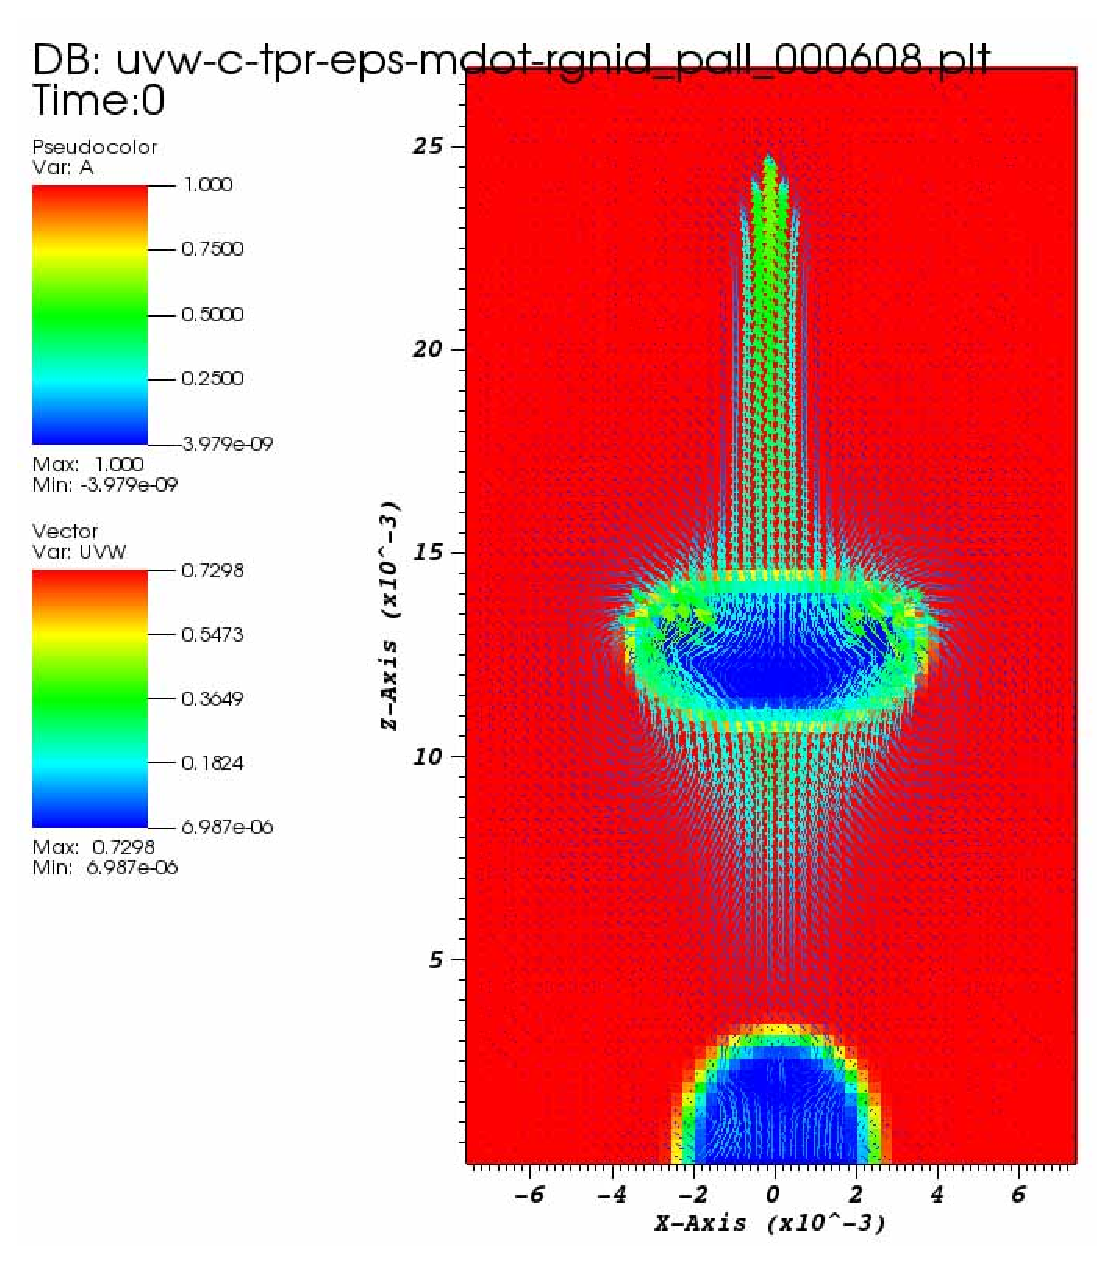
\includegraphics[scale=0.50]{Figures/10-LPT/10-11-single-phase-velocity-field.eps}}
  \end{picture}
  \caption{Single phase velocity field.}
  \label{fig_singlephasevelocityfield}
\end{figure}

%---------------------%
%                     %
%  three phase merged %
%                     %
%---------------------%
\begin{figure}[ht]
  \centering
  \setlength{\unitlength}{ 1mm}
  \begin{picture}( 60, 50)( 0, 45)
    \thickbox{ 60}{ 50}
    \put( 0, 0){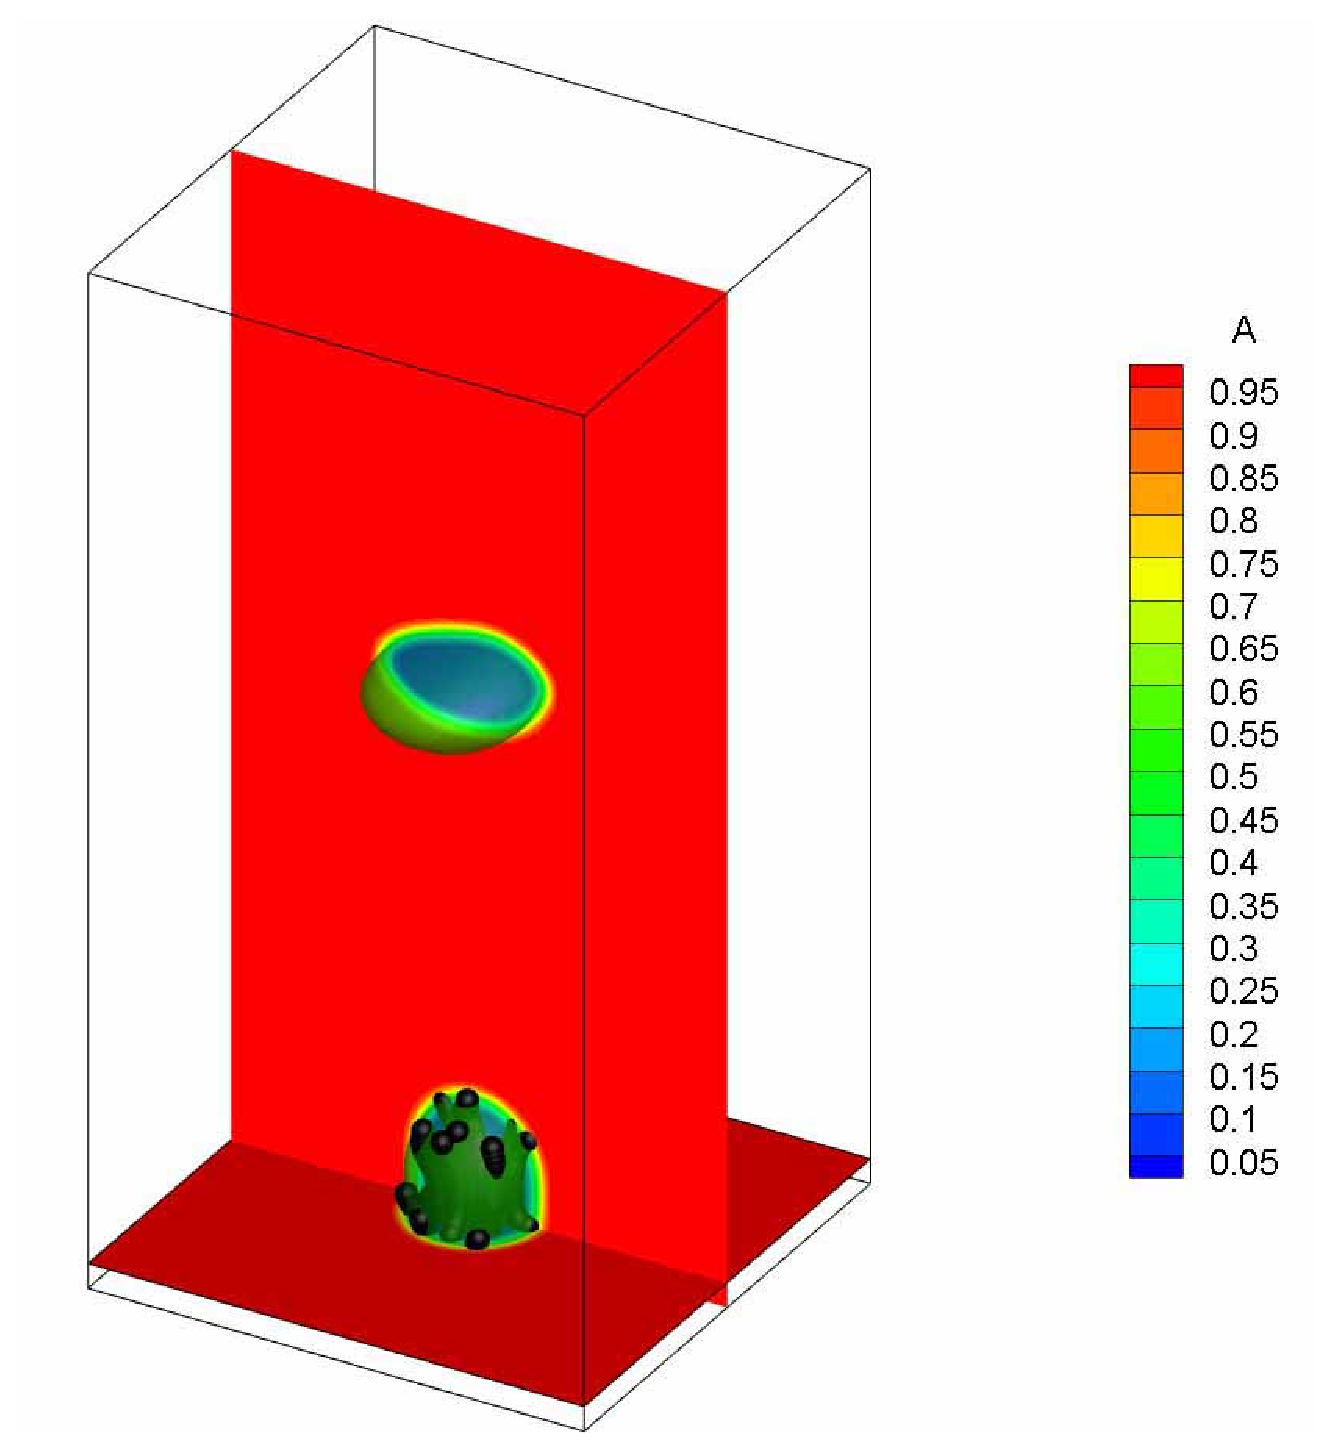
\includegraphics[scale=0.40]{Figures/10-LPT/10-12-three-phase-merged-new.eps}}
  \end{picture}
  %\caption{Three phase merged flow field.}
  \label{fig_threephasemerged}
\end{figure}

%------------------------------%
%                              %
%  three phase merged zoom in  %
%                              %
%------------------------------%
\begin{figure}[ht]
  \centering
  \setlength{\unitlength}{ 1mm}
  \begin{picture}( 100, 0)( 0, 0)
    \thickbox{ 100}{ 0}
    \put( 0, 0){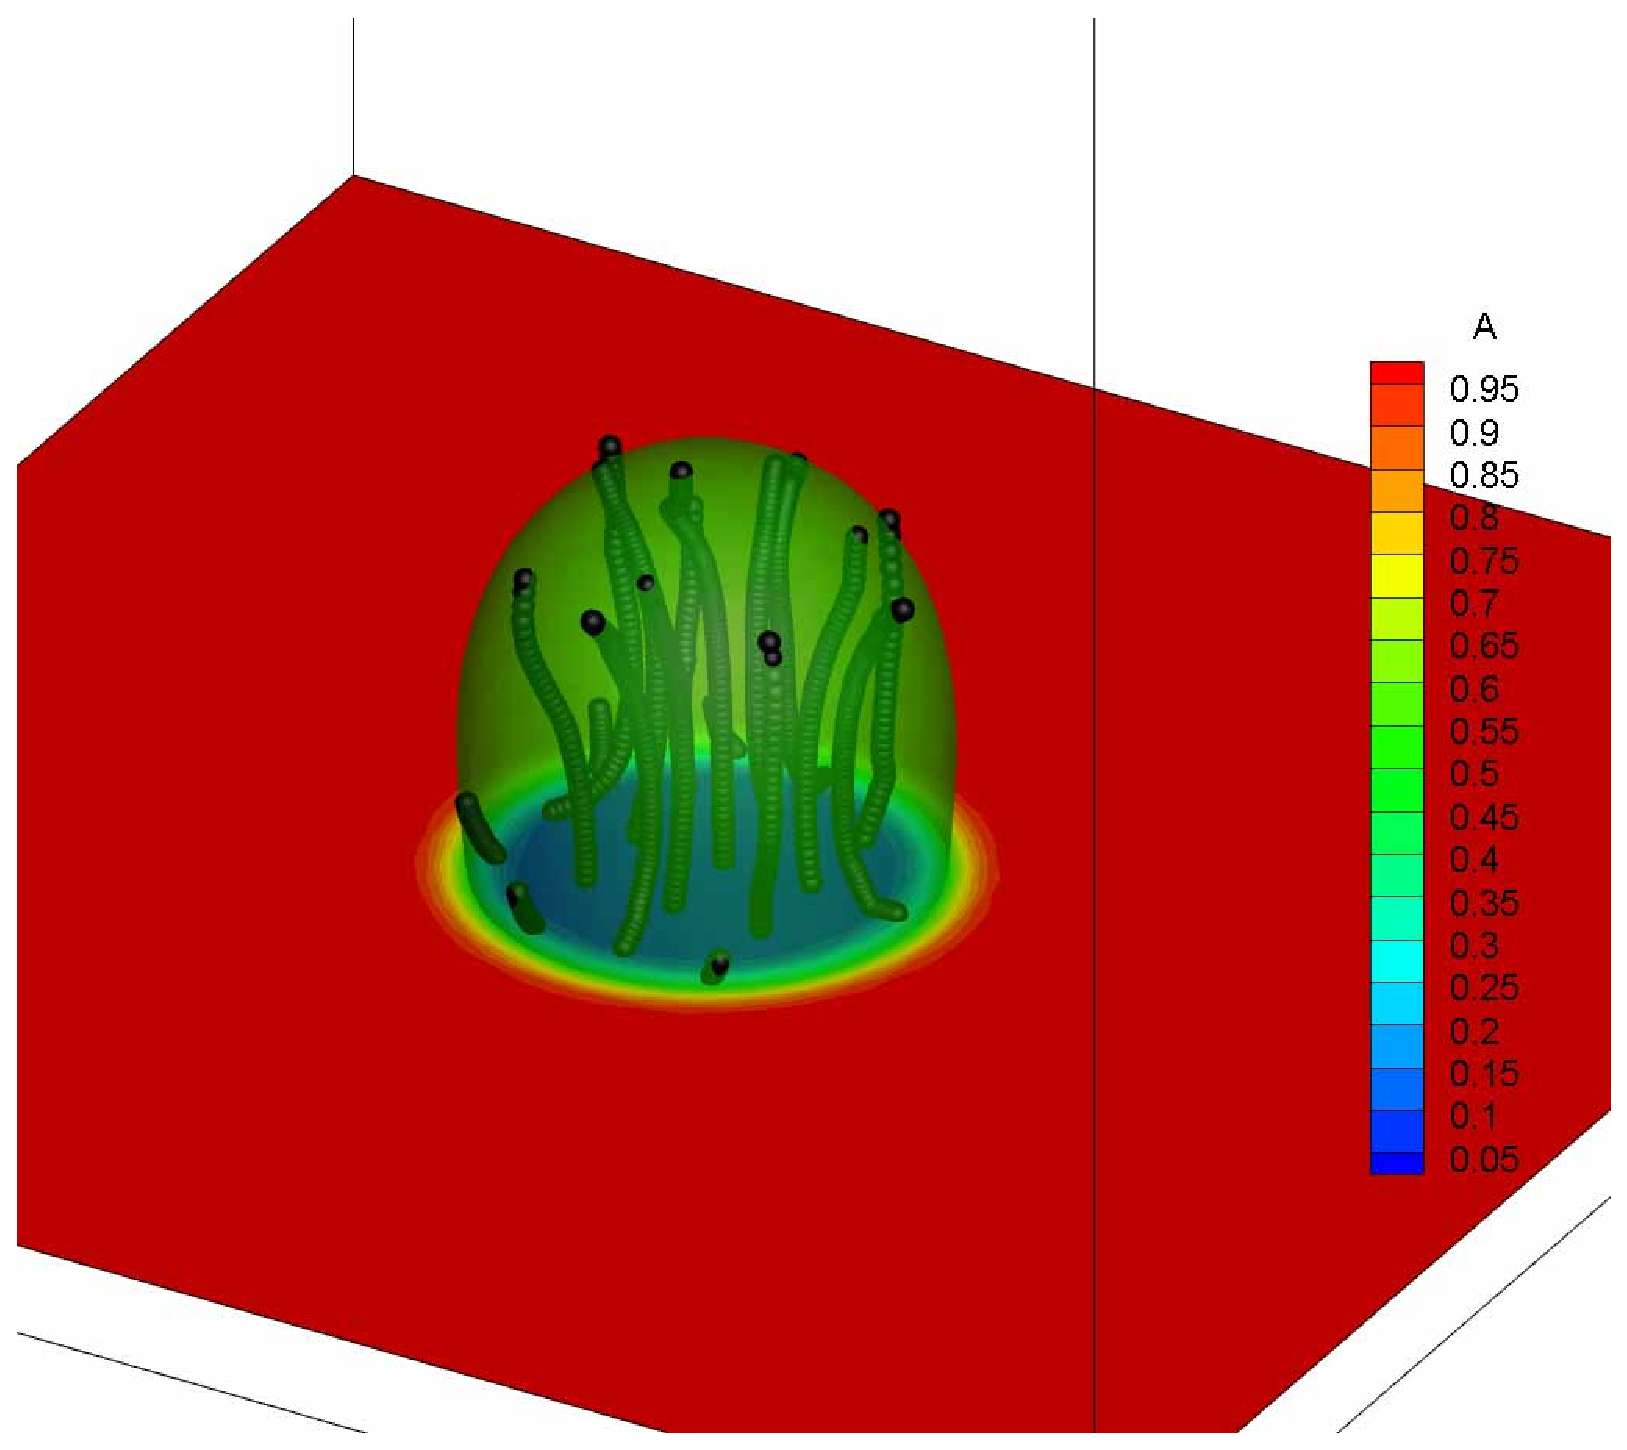
\includegraphics[scale=0.35]{Figures/10-LPT/10-13-three-phase-merged-zoom-in.eps}}
  \end{picture}
  \caption{Three phase merged flow field, zoom in.}
  \label{fig_threephasemergedzoomin}
\end{figure}
